\subsection{Graph coloring}

\begin{frame}
    \frametitle{What is a graph coloring?}
    Convert a region coloring problem to a graph coloring problem.
\begin{figure}[!h]
    \centering
    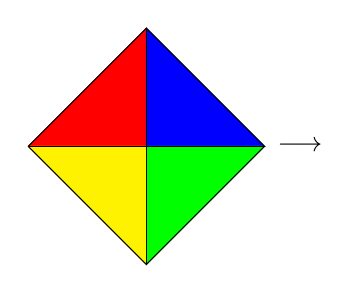
\begin{tikzpicture}[scale=1.5]
        \coordinate (v1) at (-1, 0);
        \coordinate (v2) at (0, 1);
        \coordinate (v3) at (1, 0);
        \coordinate (v4) at (0, -1);
        \coordinate (c) at (0, 0);

        \draw [fill, red] (v1) -- (v2) -- (c) -- (v1);
        \draw [fill, blue] (v2) -- (v3) -- (c) -- (v2);
        \draw [fill, green] (v3) -- (v4) -- (c) -- (v3);
        \draw [fill, yellow] (v4) -- (v1) -- (c) -- (v4);
        \draw (v1) -- (v2) -- (v3) -- (v4) -- (v1);
        \draw (c) -- (v1);
        \draw (c) -- (v2);
        \draw (c) -- (v3);
        \draw (c) -- (v4);
        \node at (1.3, 0) { $\longrightarrow$ };
    \end{tikzpicture} 
    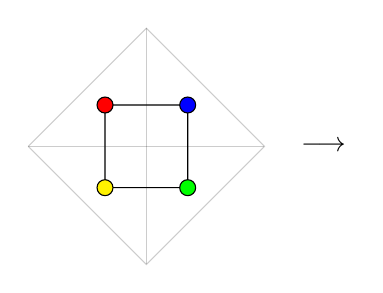
\begin{tikzpicture}[scale=1.5]
        \coordinate (v1) at (-1, 0);
        \coordinate (v2) at (0, 1);
        \coordinate (v3) at (1, 0);
        \coordinate (v4) at (0, -1);
        \coordinate (c) at (0, 0);

        \node[circle, fill, scale=0.01cm, red, draw=black] (m1) at (-0.35, 0.35) { $v_1$ };
        \node[circle, fill, scale=0.01cm, blue, draw=black] (m2) at (0.35, 0.35) { $v_2$ };
        \node[circle, fill, scale=0.01cm, green, draw=black] (m3) at (0.35, -0.35) { $v_3$ };
        \node[circle, fill, scale=0.01cm, yellow, draw=black] (m4) at (-0.35, -0.35) { $v_4$ };

        \draw (m1) -- (m2) -- (m3) -- (m4) -- (m1);
        \draw[opacity=0.2] (v1) -- (v2) -- (v3) -- (v4) -- (v1);
        \draw[opacity=0.2] (c) -- (v1);
        \draw[opacity=0.2] (c) -- (v2);
        \draw[opacity=0.2] (c) -- (v3);
        \draw[opacity=0.2] (c) -- (v4);
        \node at (1.5, 0) { $\longrightarrow$ };
    \end{tikzpicture}  
    \begin{tikzpicture}[scale=1.5, mid arrow/.style={
        postaction={ decorate, decoration={ markings, mark=at position 0.6 with { \arrow[black]{>>} } } } }]
        \coordinate (v1) at (-1, 0);
        \coordinate (v2) at (0, 1);
        \coordinate (v3) at (1, 0);
        \coordinate (v4) at (0, -1);
        \coordinate (c) at (0, 0);

        \node[circle, fill, scale=0.015cm, label=above left:$a$] (m1) at (-0.35, 0.35) { };
        \node[circle, fill, scale=0.015cm, label=above right:$b$] (m2) at (0.35, 0.35) { };
        \node[circle, fill, scale=0.015cm, label=below right:$c$] (m3) at (0.35, -0.35) { };
        \node[circle, fill, scale=0.015cm, label=below left:$d$] (m4) at (-0.35, -0.35) { };

        \draw[mid arrow] (m1) -- (m2);
        \draw (m2) -- (m3) -- (m4) -- (m1);
        \draw[opacity=0.0] (v1) -- (v2) -- (v3) -- (v4) -- (v1);
    \end{tikzpicture}     
\end{figure}
\end{frame}

\begin{frame}
    \frametitle{What is a graph coloring?}
    Problem came forth from coloring world maps.
    \includegraphics[width=\textwidth]{images/worldmap.png}
\end{frame}

\begin{frame}
    \frametitle{The Four Color Theorem}
    \begin{theorem}
        Every planar graph can be colored in at most four colors.
    \end{theorem}

    A simple statement. First formulated in 1852, proven over a hundred years later in 1976. 
\end{frame}

\begin{frame}
    \frametitle{The Five Color Theorem}
    \begin{theorem}<1->
        Every planar graph can be colored in at most five colors.
    \end{theorem}
    \begin{proof}<2->
            Every planar graph $G$ has a vertex of $\deg(v)\leq 5$.
            \begin{itemize}
                \item If $\deg(v) \leq 4$, can use fifth color.
                \item If $\deg(v) = 5$, can always free up a color.
            \end{itemize}
            Remove $v$ from the graph and repeat until there are no vertices left. Add back and color these vertices until we obtain a coloring of $G$.
    \end{proof}
\end{frame}

\begin{frame}
    \frametitle{The Five Color Theorem}
    \begin{alertblock}{Most important argument}
        If $\deg(v)=5$, can always free up a color.
    \end{alertblock}
    \vspace{0.5cm}
    \begin{minipage}{0.59\textwidth}
        \begin{itemize}
            \item If there is an $ac$-chain, then we have isolated $b$. Therefore, there can not be a $bd$-chain from $b$ to $d$. We may flip the $bd$-chain of $b$ to free up the color $d$. 
            \item If there is no $ac$-chain, then $a$ and $c$ are not connected. So we may flip the $ac$-chain of $a$ to free up the color $c$.
        \end{itemize}
    \end{minipage}
    \begin{minipage}{0.39\textwidth}
        \centering
        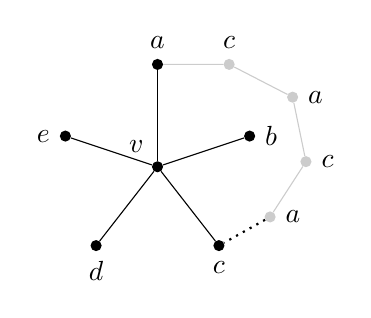
\begin{tikzpicture}[scale=1.3]
            \node[circle, fill, scale=0.015cm, label=above left:$v$] (c) at (0, 0) {};
            \node[circle, fill, scale=0.015cm, label=above:$a$] (l1) at (0, 1) { };
            \node[circle, fill, scale=0.015cm, label=right:$b$] (l2) at (0.9, 0.30) { };
            \node[circle, fill, scale=0.015cm, label=below:$c$] (l3) at (0.6, -0.77) {};
            \node[circle, fill, scale=0.015cm, label=below:$d$] (l4) at (-0.6, -0.77) {};
            \node[circle, fill, scale=0.015cm, label=left:$e$] (l5) at (-0.9, 0.30) {};
            \node[circle, fill, scale=0.015cm, label=above:$c$, opacity=0.2] (c1) at (0.7, 1) {};
            \node[circle, fill, scale=0.015cm, label=right:$a$, opacity=0.2] (c2) at (1.32, 0.68) {};
            \node[circle, fill, scale=0.015cm, label=right:$c$, opacity=0.2] (c3) at (1.45, 0.05) {};
            \node[circle, fill, scale=0.015cm, label=right:$a$, opacity=0.2] (c4) at (1.1, -0.49) {};
    
            \draw (c) -- (l1);
            \draw (c) -- (l2);
            \draw (c) -- (l3);
            \draw (c) -- (l4);
            \draw (c) -- (l5);
    
            \draw[opacity=0.2] (l1) -- (c1) -- (c2) -- (c3) -- (c4);
            \draw[dotted, thick] (c4) -- (l3);
            
        \end{tikzpicture}
    \end{minipage}
\end{frame}
\subsection{Fundaments of the four color theorem}

The proof of the four color theorem follows the same structure as the five color theorem. We show that every planar graph contains a subgraph that allows us to reduce the coloring problem to a smaller graph. This notion of a \textit{subgraph} of a graph requires some extra attention, since there are multiple ways to be a subgraph.

Given a subgraph $\confg$ of a planar graph $G$. There are roughly two ways that $\confg$ can be a subgraph of $G$. See Figure \ref{fig:containtut}.

\begin{figure}[!ht]
    \centering
    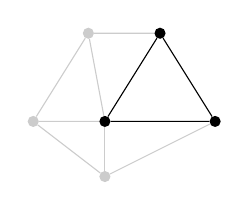
\begin{tikzpicture}[scale=0.7]
        \node[circle, fill, scale=0.015cm] (l1) at (-1, 0) { };
        \node[circle, fill, scale=0.015cm] (l2) at (1, 0) { };
        \node[circle, fill, scale=0.015cm] (l3) at (0, 1.6) {};

        \node[circle, fill, scale=0.015cm, opacity=0.2] (e1) at (-1.3, 1.6) { };
        \node[circle, fill, scale=0.015cm, opacity=0.2] (e2) at (-2.3, 0) { };
        \node[circle, fill, scale=0.015cm, opacity=0.2] (e3) at (-1, -1) { };

        \draw (l1) -- (l2) -- (l3) -- (l1);
        \draw[opacity=0.2] (e1) -- (l1) -- (e2);
        \draw[opacity=0.2] (e3) -- (l1);
        \draw[opacity=0.2] (l3) -- (e1) -- (e2) -- (e3) -- (l2);
    \end{tikzpicture}
    \hspace{1cm}
    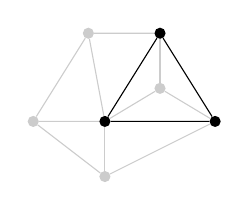
\begin{tikzpicture}[scale=0.7]
        \node[circle, fill, scale=0.015cm] (l1) at (-1, 0) { };
        \node[circle, fill, scale=0.015cm] (l2) at (1, 0) { };
        \node[circle, fill, scale=0.015cm] (l3) at (0, 1.6) {};

        \node[circle, fill, scale=0.015cm, opacity=0.2] (e1) at (-1.3, 1.6) { };
        \node[circle, fill, scale=0.015cm, opacity=0.2] (e2) at (-2.3, 0) { };
        \node[circle, fill, scale=0.015cm, opacity=0.2] (e3) at (-1, -1) { };

        \node[circle, fill, scale=0.015cm, opacity=0.2] (w1) at (0, 0.6) { };

        \draw (l1) -- (l2) -- (l3) -- (l1);
        \draw[opacity=0.2] (w1) -- (l1);
        \draw[opacity=0.2] (w1) -- (l2);
        \draw[opacity=0.2] (w1) -- (l3);
        \draw[opacity=0.2] (e1) -- (l1) -- (e2);
        \draw[opacity=0.2] (e3) -- (l1);
        \draw[opacity=0.2] (l3) -- (e1) -- (e2) -- (e3) -- (l2);
    \end{tikzpicture}
    \caption{A configuration contained in a graph (left). No containmnet (right).}
    \label{fig:containtut}
\end{figure}

\begin{definition}
    A planar graph $\confg$ is \emph{contained} in a graph $G$ if no vertices of $G$ are in the interior of $\confg$.
\end{definition}

\begin{definition}
    A planar graph $\confg$ is \emph{reducible} in a graph $G$ if $\confg$ being contained in $G$ implies that the 4-coloring of $G$ can be reduced to the 4-coloring of $G'$ with less vertices. $\confg$ is called a \emph{configuration}.
\end{definition}

Using these two definitions we can formulate the key theorem of the four color theorem. It simply states that every planar graph has a part that can be removed and recolored later, similar to how we did for the five color theorem.

\begin{theorem}
    \label{funda1}
    Every planar graph $G$ contains a configuration $\confg$ that is either $k$-reducible, D-reducible or C-reducible in $G$.
\end{theorem}

From this theorem, a 4-coloring of a planar graph $G_0$ can be found as follows. This is the same procedure that we used for the vertex of $\deg(v)\leq 5$ in the five color theorem.

\begin{enumerate}
    \item Find a reducible configuration $C_n$ in $G_n$.
    \item Reduce the graph $G_n$ to the smaller graph $G_{n+1}$.
    \item If $G_{n+1}$ is the empty graph, color all the intermediate graphs starting from $G_n$ all the way until $G_0$, else, repeat Step 1 on $G_{n+1}$.
\end{enumerate}